\documentclass[a4paper]{article}
\usepackage[utf8]{vietnam}
\usepackage[left=3.5cm,right=2.5cm,top=2cm,bottom=2cm]{geometry} 
\usepackage[utf8]{inputenc}
\usepackage{arxiv}
\usepackage{graphicx}
\usepackage{minted}
\usepackage{float}
\usepackage[utf8]{inputenc} % allow utf-8 input
\usepackage[utf8]{vietnam}
\usepackage[left=3.5cm,right=2.5cm,top=2cm,bottom=2cm]{geometry} 
\usepackage{varioref}
\usepackage[hidelinks]{hyperref}
\usepackage[nameinlink, capitalise, noabbrev]{cleveref}
\setlength{\parindent}{0pt}
%\usepackage{wallpaper}
%\usepackage[firstpage]{draftwatermark} 
\usepackage{xcolor}
\definecolor{LightGray}{gray}{1.0}
\usepackage{tikz} 
\usepackage{scrextend}
%\usepackage{background}
\usetikzlibrary{calc}
\usepackage{xcolor}
\usepackage{minted}
\usepackage[vietnamese]{babel}
\usepackage{amsmath}
\usepackage[T1]{fontenc}    % use 8-bit T1 fonts
\usepackage{hyperref}       % hyperlinks
\usepackage{url}            % simple URL typesetting
\usepackage{booktabs}       % professional-quality tables
\usepackage{amsfonts}       % blackboard math symbols
\usepackage{nicefrac}       % compact symbols for 1/2, etc.
\usepackage{microtype}      % microtypography
\usepackage{natbib}
\usepackage{titlesec}
\usepackage{multicol}
\usepackage{color}
\usepackage{algorithm}
\usepackage{algpseudocode}
\setlength{\columnseprule}{1pt}
\titleformat*{\section}{\Large\bfseries}
\titleformat*{\subsection}{\Large\bfseries}
\titleformat*{\subsubsection}{\large\bfseries}
\titleformat*{\paragraph}{\large\bfseries}
\titleformat*{\subparagraph}{\large\bfseries}
\begin{document}

\begin{titlepage}

%\SetWatermarkText{\includegraphics[width = 0.97\paperwidth,
%height = 0.97\paperheight]{bia.png}}
%\SetWatermarkAngle{0} 
%\SetWatermarkText{\includegraphics[scale=1]{hust.png}}
%\SetWatermarkAngle{0} 
\begin{tikzpicture}[remember picture,overlay,inner sep=0,outer sep=0]
    \definecolor{codegreen}{rgb}{71,136,101}
     \draw[teal!70!black,line width=4pt] ([xshift=-1.5cm,yshift=-2cm]current page.north east) coordinate (A)--([xshift=1.5cm,yshift=-2cm]current page.north west) coordinate(B)--([xshift=1.5cm,yshift=2cm]current page.south west) coordinate (C)--([xshift=-1.5cm,yshift=2cm]current page.south east) coordinate(D)--cycle;

     \draw ([yshift=0.5cm,xshift=-0.5cm]A)-- ([yshift=0.5cm,xshift=0.5cm]B)--
     ([yshift=-0.5cm,xshift=0.5cm]B) --([yshift=-0.5cm,xshift=-0.5cm]B)--([yshift=0.5cm,xshift=-0.5cm]C)--([yshift=0.5cm,xshift=0.5cm]C)--([yshift=-0.5cm,xshift=0.5cm]C)-- ([yshift=-0.5cm,xshift=-0.5cm]D)--([yshift=0.5cm,xshift=-0.5cm]D)--([yshift=0.5cm,xshift=0.5cm]D)--([yshift=-0.5cm,xshift=0.5cm]A)--([yshift=-0.5cm,xshift=-0.5cm]A)--([yshift=0.5cm,xshift=-0.5cm]A);


     \draw ([yshift=-0.3cm,xshift=0.3cm]A)-- ([yshift=-0.3cm,xshift=-0.3cm]B)--
     ([yshift=0.3cm,xshift=-0.3cm]B) --([yshift=0.3cm,xshift=0.3cm]B)--([yshift=-0.3cm,xshift=0.3cm]C)--([yshift=-0.3cm,xshift=-0.3cm]C)--([yshift=0.3cm,xshift=-0.3cm]C)-- ([yshift=0.3cm,xshift=0.3cm]D)--([yshift=-0.3cm,xshift=0.3cm]D)--([yshift=-0.3cm,xshift=-0.3cm]D)--([yshift=0.3cm,xshift=-0.3cm]A)--([yshift=0.3cm,xshift=0.3cm]A)--([yshift=-0.3cm,xshift=0.3cm]A);

   \end{tikzpicture}
   
\begin{center}
    \vspace{7pt}
    \large
    \textbf{BỘ GIÁO DỤC VÀ ĐÀO TẠO}\\
    \vspace{7pt}
    \textbf{TRƯỜNG ĐẠI HỌC KINH TẾ THÀNH PHỐ HỒ CHÍ MINH}\\
    \vspace{7pt}
    \textbf{TRƯỜNG CÔNG NGHỆ VÀ THIẾT KẾ}
\end{center}
\vspace{10pt}
\begin{center}
    
\includegraphics[scale=0.3]{ueh.jpeg}
    
    \vspace{20pt}
    \fontsize{14pt}{13pt}\selectfont 
    \textbf{ĐỒ ÁN MÔN HỌC} 
    
    \vspace{7pt}
    {CƠ SỞ LẬP TRÌNH}
\end{center}

\vspace{3cm}
\large
\begin{center}
    \textbf{Sinh viên}: NGUYỄN QUỐC VIỆT\\
    \vspace{7pt}
    \textbf{Chuyên ngành}: KHOA HỌC DỮ LIỆU\\
    \vspace{7pt}
    \textbf{Khoá}: K47
\end{center}

\vspace{2cm}
\large
\begin{center}
    \textbf{Giảng viên:} TS. Đặng Ngọc Hoàng Thành
\end{center}
\vfill
\large
\begin{center}
    \textbf{TP Hồ Chí Minh, 2022}
\end{center}
\end{titlepage}

\large
\tableofcontents
\vfill

\section{ĐỀ BÀI}
\subsection{Phần 1}
Viết chương trình mô phỏng trò chơi Bao – Búa – Kéo. Biết:Bao thắng  Búa, Búa thắng Kéo, Kéo thắng Bao.

\subsection{Phần 2} 
$$
P=\frac{1}{\sqrt[n+1]{1+\sqrt[n+1]{2+\sqrt[n+1]{3+\cdots+\sqrt[n+1]{n+1}}}}}
$$
Có $n+1$ dấu căn. Trong đó $n$ là số thứ tự của tên bạn trong danh sách, ví dụ, bạn có số thứ tự là 1,11,21,... thì $n=1$, như yêu cầu đầu tiên.\\

\subsection{Phần 3}
Nhập các hệ số của đa thức bậc $n$ theo $x$ vào một mảng. Nhập giá trị $X$. In ra kết quả đa thức này.
$$
F(x) = a_{n}x^{n} + a_{n-1}x^{n-1} + ... + a_{2}x^{2} + a_{1}x + a_{0}
$$

\subsection{Phần 4}
Nhập các phần tử của ma trận $A_{m \times n}$, kiểm tra ma trận này có phải là ma trận đối xứng qua trục giữa không?\\

\subsection{Phần 5}
Nhập chuỗi S, chuỗi con s1 và chuỗi con s2. Thay thế tất cả chuỗi s1 thành chuỗi s2 trong chuỗi S.\\

Ví dụ \texttt{S=”Bong chang chon luot qua ngon che”; s1=”ch”; s2=”tr”}\\

Kết quả in ra \texttt{“Bong trang tron luot qua ngon tre”}\\

\subsection{Phần 6}
Cho một mảng nhiều chiều gồm thông tin cá nhân của mỗi sinh viên: họ tên, năm sinh, điểm trung bình, xếp loại. Giả sử dữ liệu của mảng gồm có ít nhất 5 phần tử. Hãy in ra toàn bộ các phiếu điểm theo mẫu như sau:\\
\pagebreak
\texttt{--------------------------------- \\
BẢNG ĐIỂM TỐT NGHIỆP\\
Cấp cho sinh viên <họtên>, năm sinh <năm sinh>.\\
Trong kì thi tốt nghiệp 2021, sinh viên trên đã đạt điểm trung bình là <điểm trung bình>, và được xếp loại <xếp loại>.Sinh viên có thứ hạng <???> trong lớp.\\
Hiệu Trưởng Trường Đại học ABC.\\
Kí tên, Đóng dấu\\
--------------------------------- \\}
\vfill
\pagebreak
\section{LỜI GIẢI}
\subsection{Bài 1}
\subsubsection{Phân tích}
\begin{itemize}
    \item Nếu người chơi và máy tính chọn giống nhau thì xuất kết quả "Hoà". 
    \item Nếu người chơi ra Kéo thì 
    \begin{itemize}
        \item Thông báo "Người chơi thắng" nếu máy tính ra Bao
        \item Ngược lại thông báo người chơi thua
    \end{itemize}
    \item Nếu người chơi ra Bao thì
    \begin{itemize}
        \item Thông báo "Người chơi thắng" nếu máy tính ra Búa
        \item Ngược lại thông báo người chơi thua
    \end{itemize}
    \item Nếu người chơi ra Búa thì
    \begin{itemize}
        \item Thông báo "Người chơi thắng" nếu máy tính ra Kéo
        \item Ngược lại thông báo người chơi thua
    \end{itemize}
\end{itemize}
\subsubsection{Thuật toán}
a) Mô tả thuật toán
\begin{enumerate}
    \item Khởi gán lựa chọn của máy tính (ComputerChoice) bằng một giá trị số nguyên bất kì nằm trong khoảng (1,3), đại diện cho Kéo, Búa, Bao, cụ thể:
    \begin{itemize}
        \item 1: Kéo
        \item 2: Búa
        \item 3: Bao
    \end{itemize}
    
    \item Nếu lựa chọn không hợp lệ thì xuất kết quả “Lựa chọn không hợp lệ. Chỉ chấp nhận lựa chọn là số nguyên từ 1-3. Vui lòng chọn lại”. Nếu lựa chọn hợp lại thì thực hiện bước tiếp theo.
    
    \item Gọi (ComputerChoice, PlayerChoice) là các cặp số nguyên khả thi. Thực thi câu lệnh if:  
    \begin{itemize}
        \item Nếu ComputerChoice = PlayerChoice thì xuất kết quả Hoà.
        
        \item Xuất kết quả “Người chơi thắng” trong khi có các bộ số sau: $(3,1),(1,2)$ và $(2,3)$.
        
        \item Ngược lại thì xuất kết quả “Người chơi thua”.
    \end{itemize}
\end{enumerate}

\begin{algorithm}
\caption{Thuật toán trò chơi kéo búa bao}\label{alg:cap}
\begin{algorithmic}
\Require $1 \leq n \leq 3$

\If{PlayerChoice == ComputerChoice}
    \State ketqua = "Hoà"
\ElsIf{PlayerChoice \& ComputerChoice in [(1,3),(2,1),(3,2)]}
    \State ketqua = "Thắng"
\Else   
    \State ketqua = "Thua"
\EndIf\\
\Return ketqua
\end{algorithmic}
\end{algorithm}
\vfill
b) Sơ đồ khối
\begin{figure}[!h]
    \centering
    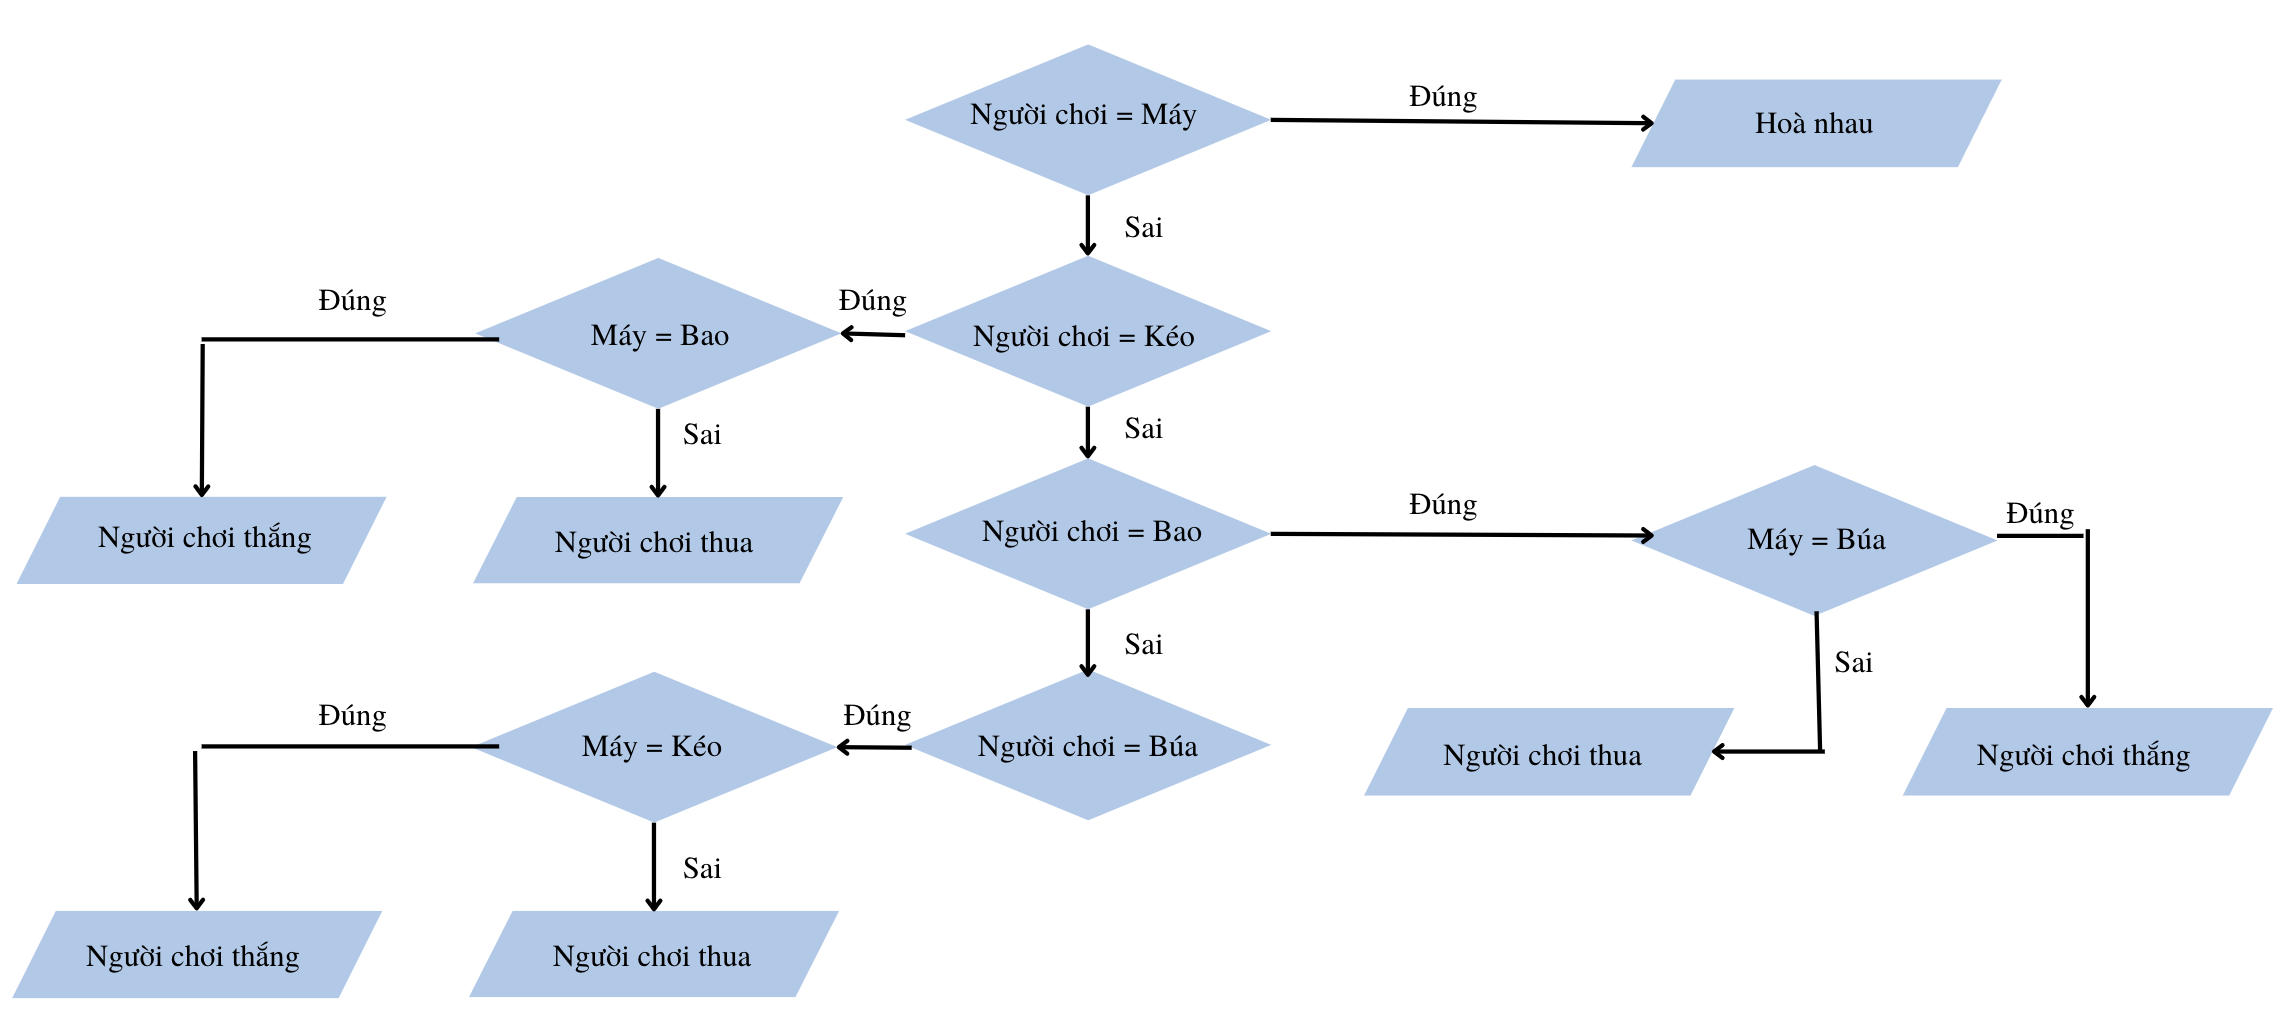
\includegraphics[width=17cm]{diagram.png}
    \caption{Sơ đồ khối trò chơi kéo búa bao}
    \end{figure}
    
c) Mã nguồn
\begin{minted}
[tabsize=2,breaklines,frame=lines,framesep=2mm,baselinestretch=1.2, bgcolor=LightGray, fontsize=\small, linenos]
{csharp}
        static void bai1()
        {
            Console.Clear();
            Console.WriteLine("KÉO - BÚA  - BAO\n");
            int Computer = new Random().Next(1, 3);
            string ComputerChoiceName = Computer == 1 ? "Kéo" : Computer == 2 ? "Búa" : "Bao";
        reinput1_1:
            Console.WriteLine("Nhập lựa chọn của bạn:");
            Console.WriteLine("[1] Kéo\t[2] Búa\t[3] Bao\t");
            ConsoleKeyInfo key;
            int Player;
            key = Console.ReadKey(true);
            string num = key.KeyChar.ToString();
            if (int.TryParse(num, out Player) == false)
            {
                Console.Clear();
                Console.WriteLine("Lựa chọn của bạn không tồn tại. Chỉ chấp nhận lựa chọn là số nguyên từ 1-3. Vui lòng chọn lại.");
                goto reinput1_1;
            }
            string PlayerChoiceName = Player== 1 ? "Kéo" : Player == 2 ? "Búa" : Player == 3 ? "Bao" : "";
            if (Player > 0 & Player < 4)
                if (Player == Computer)
                    Console.WriteLine("Lựa chọn của bạn là {0}, lựa chọn của máy là {1}. Kết quả: Hòa", PlayerChoiceName, ComputerChoiceName);
                else
                    if (Player == 1 & Computer == 3 || Player == 2 & Computer == 1 || Player == 3 & Computer == 2)
                    Console.WriteLine("Lựa chọn của bạn là {0}, lựa chọn của máy là {1}. Kết quả: Bạn thắng", PlayerChoiceName, ComputerChoiceName);
                else Console.WriteLine("1Lựa chọn của bạn là {0}, lựa chọn của máy là {1}. Kết quả: Máy thắng", PlayerChoiceName, ComputerChoiceName);
            else
            {
                Console.Clear();
                Console.WriteLine("Lựa chọn của bạn không tồn tại. Chỉ chấp nhận lựa chọn là số nguyên từ 1-3. Vui lòng chọn lại.");
                goto reinput1_1;
            }
        }
\end{minted}
\subsection{Bài 2}
\subsubsection{Phân tích}
Sử dụng vòng lặp \texttt{for} để thực hiện phép tính biểu thức:
$$
P=\frac{1}{\sqrt[n+1]{1+\sqrt[n+1]{2+\sqrt[n+1]{3+\cdots+\sqrt[n+1]{n+1}}}}}
$$
với $n$ là số nguyên do người dùng nhập vào.
\subsubsection{Thuật toán}
a) Mô tả thuật toán
\begin{enumerate}
    \item Yêu cầu người dùng nhập vào số thứ tự có dạng số nguyên $n$. Xuất thông báo "Chỉ chấp nhận số nguyên dương khác 0. Vui lòng nhập lại." nếu dữ liệu đầu vào không hợp lệ. Ngược lại thực hiện bước tiếp theo.
    \item Lấy số cuối cùng của số thứ tự bằng cách thực hiện phép chia lấy phần dư. 
    \item Dùng vòng lặp \texttt{for} để tính giá trị biểu thức, với \texttt{i>1} và i giảm dần (\texttt{i--}).
\end{enumerate}


\begin{algorithm}
\caption{Thuật toán tính biểu thức $P$}\label{alg:cap}
\begin{algorithmic}
\If{\texttt{sothutu} > 0}
\State n = \texttt{sothutu} \% 10 + 1
\Else
\State "Mời nhập lại"
\EndIf\\
\For{{$i=n$ down to 1}}
        \State $P_1 = [(i-1)+P_1]^\frac{1}{n}$
      \EndFor\\
\Return $P_1$
\end{algorithmic}
\end{algorithm}

b) Mã nguồn
\begin{minted}
[tabsize=2,breaklines,frame=lines,framesep=2mm,baselinestretch=1.2, bgcolor=LightGray, fontsize=\footnotesize, linenos]
{csharp}
static void bai2()
        {
            Console.Clear();
        reinput2_1:
            Console.Write("Nhập vào số thứ tự: ");
            string num = Console.ReadLine();
            int stt;
            if (int.TryParse(num, out stt) == false)
            {
                Console.WriteLine("Chỉ chấp nhận số nguyên dương khác 0. Vui lòng nhập lại.");
                goto reinput2_1;
            }
            if (stt <= 0)
            {
                Console.WriteLine("Chỉ chấp nhận số nguyên dương khác 0. Vui lòng nhập lại.");
                goto reinput2_1;
            }
            int n = stt % 10 + 1;
            Console.WriteLine("Số thứ tự {0} => có {1} dấu căn.\n", stt,n);
            double P1 = Math.Pow(n, 1 / (double)n);
            for (int i = n; i > 1; i--)
                P1 = Math.Pow((i - 1) + P1, 1 / (double)n);
            Console.WriteLine("Kết Quả: {0}", 1 / P1);
        }
\end{minted}
\subsection{Bài 3}
\subsubsection{Phân tích}
Sử dụng vòng lặp \texttt{for} tính giá trị của biểu thức có $n$ bậc có dạng
$$
F(x) = a_{n}x^{n} + a_{n-1}x^{n-1} + ... + a_{2}x^{2} + a_{1}x + a_{0}
$$
\subsubsection{Thuật toán}
a) Mô tả thuật toán
\vspace{-10pt}
\begin{enumerate}
    \item Yêu cầu người dùng nhập vào bậc n cao nhất của đa thức cần tính. Nếu lựa chọn không hợp lệ thì xuất kết quả "Chỉ chấp nhận số nguyên dương khác 0. Vui lòng nhập lại." Ngược lại ta thực hiện bước tiếp theo.
    \item Sử dụng vòng lặp for, khởi gán $i = n,$ điều kiện dừng $i > 0$. Yêu cầu người dùng nhập vào các hệ số tương ứng cho từng bậc $n, n-1, …$. và hệ số tự do. Nếu lựa chọn không hợp lệ thì xuất kết quả ""Nhập sai. Chỉ chấp nhận số. Vui lòng nhập lại.." Ngược lại ta thực hiện bước tiếp theo.
    \item Yêu cầu người dùng nhập vào giá trị của x. Thực hiện phép tính ở bước tiếp theo, nếu input không hợp lệ thì xuất thông báo “"Nhập sai. Chỉ chấp nhận số. Vui lòng nhập lại.”
    \item Sủ dụng vòng lặp for, với mỗi giá trị, tính giá trị $result = result + F[i] + X^{i}$
\end{enumerate}

\begin{algorithm}
\caption{Thuật toán tính biểu thức $F(x)$}\label{alg:cap}
\begin{algorithmic}
\Require $degree > 0$
\Require $X$

\For{{i=level down to 0}}
        \State Nhập vào hệ số của hạng bậc $i$
      \EndFor\\
\For{{i=level,, i down to 0}}
        \State {$result = result + F_{i} + X^{i}$}
    \EndFor\\
\Return $result$
\end{algorithmic}
\end{algorithm}
\pagebreak
b) Mã nguồn
\begin{minted}
[tabsize=2,breaklines,frame=lines,framesep=2mm,baselinestretch=1.2, bgcolor=LightGray, fontsize\footnotesize, linenos]
{csharp}
        static void bai3()
        {
            Console.Clear();
        reinput3_1:
            Console.Write("Nhập vào bậc của đa thức: ");
            string num = Console.ReadLine();
            int level;
            if (int.TryParse(num, out level) == false)
            {
                Console.WriteLine("Chỉ chấp nhận số nguyên dương khác 0. Vui lòng nhập lại.");
                goto reinput3_1;
            }
            if (level <= 0)
            {
                Console.WriteLine("Chỉ chấp nhận số nguyên dương khác 0. Vui lòng nhập lại.");
                goto reinput3_1;
            }
            double[] F = new double[level + 1];
            for (int i = level; i > 0; i--)
            {
            reinput3_2:
                Console.Write("Nhập vào hệ số của số hạng bậc {0}: ", i);
                num = Console.ReadLine();
                if (double.TryParse(num, out F[i]) == false)
                {
                    Console.WriteLine("Nhập sai. Chỉ chấp nhận số. Vui lòng nhập lại.");
                    goto reinput3_2;
                }
            }
        reinput3_3:
            Console.Write("Nhập vào hệ số tự do: ");
            num = Console.ReadLine();
            if (double.TryParse(num, out F[0]) == false)
            {
                Console.WriteLine("Nhập sai. Chỉ chấp nhận số. Vui lòng nhập lại.");
                goto reinput3_3;
            }
        reinput3_4:
            Console.Write("Nhập vào giá trị của X: ");
            num = Console.ReadLine();
            if (double.TryParse(num, out double X) == false)
            {
                Console.WriteLine("Nhập sai. Chỉ chấp nhận số. Vui lòng nhập lại.");
                goto reinput3_4;
            }
            double result = 0;
            for (int i = level; i >= 0; i--)
                result = result + F[i] * Math.Pow(X, i);
            Console.WriteLine("Kết quả: {0}", result);
        }
\end{minted}
\subsection{Bài 4}
\subsubsection{Phân tích}
Dùng vòng lặp for, kiểm tra phần tử $a[i]$ và với giá trị tương ứng (đối xứng qua trục dọc, trục ngang). Nếu bằng nhau thì ma trận là đối xứng qua trục giữa, ngược lại ma trận không đối xứng.\\

Ví dụ: Kiểm tra tính đối xứng qua trục giữa của ma trận:

$ \mathbf{A} = \begin{bmatrix}
1 & 3 & 4 & 1 \\
2 & 4 & 4 & 2 \\
3 & 4 & 5 & 3 \\
4 & 5 & 6 & 4 
\end{bmatrix}  $

Kiểm tra từ vị trí của phần tử đầu tiên $A_{0,0} =1$ với phần tử tương ứng $A_{4,3}$, với:
\begin{itemize}
    \item 4 là số phần tử của hàng $i$
    \item 3 được tính bằng cách lấy số phần tử hàng $i - 1 - index$ của giá trị $i$ đang xét: $4 - 1 - 0 = 3$
\end{itemize}

Ta thấy cả bốn phần tử đều bằng nhau nên ma trận $\mathbf{A}$ đối xứng qua trục dọc. 
\subsubsection{Thuật toán}
a) Mô tả thuật toán
\begin{enumerate}
    \item Khai báo mảng hai chiều \texttt{double a}. Yêu cầu người dùng nhập vào từng phần tử tương ứng.
    \item Kiểm tra đối xứng qua trục dọc. Với mỗi $i = 0$ và $i <$ tổng số phần tử của hàng, với mỗi $j$, thực hiện:
    \begin{itemize}
        \item Kiểm tra phần tử \texttt{a[i][j]} với phần tử tương ứng đối xứng qua trục dọc là \texttt{a[i][Số phần tử của hàng - 1 - j]}. Nếu có cặp hai giá trị không bằng nhau thì xuất thông báo " Ma trận không đối xứng qua trục dọc", ngược lại xuất thông báo "Ma trận đối xứng qua trục dọc"
        \item Kiểm tra phần tử \texttt{a[i][j]} với phần tử tương ứng đối xứng qua trục ngang là \texttt{a[Số phần tử của hàng - 1 - j][i]}. Nếu có cặp hai giá trị không bằng nhau thì xuất thông báo " Ma trận không đối xứng qua trục ngang", ngược lại xuất thông báo "Ma trận đối xứng qua trục ngang"
    \end{itemize}
\end{enumerate}

\begin{algorithm}
\caption{Thuật toán kiểm tra tính đối xứng của ma trận}\label{alg:cap}
\begin{algorithmic}
\Require Số dòng của ma trận $sizeM$
\Require Số cột của ma trận $sizeN$
\Require Các phần tử $a_{ij}$ của ma trận

\Comment{Kiểm tra đối xứng trục dọc}
\For{i=0 up to number of rows}
    \For{j=0 up to number of columns}
        \If{$a_{[ij]} \# a_{[i][a_{i} - 1 - j]}$}
            \State Ma trận đối xứng qua trục dọc
        \Else
            \State pass
        \EndIf
    \EndFor
\EndFor

\Comment{Kiểm tra đối xứng trục ngang}
\For{i=0 up to number of columns}
    \For{j=0 up to number of rows}
        \If{$a_{[ij]} \# a_{[Số phần tử của hàng - 1 - j][i]}$}
            \State Ma trận đối xứng qua trục ngang
        \Else
            \State pass
        \EndIf
    \EndFor
\EndFor
\end{algorithmic}
\end{algorithm}

b) Mã nguồn
\begin{minted}
[tabsize=2,breaklines,frame=lines,framesep=2mm,baselinestretch=1.2, bgcolor=LightGray, fontsize=\footnotesize, linenos]
{csharp}
        static void buildmatrix(double[][] a)
        {
            for (int i = 0; i < a.Length; i++)
                for (int j = 0; j < a[i].Length; j++)
                {
                reinput4_3:
                    Console.Write("Nhập vào phần tử [{0},{1}]: ", i, j);
                    string num = Console.ReadLine();
                    if (double.TryParse(num, out a[i][j]) == false)
                    {
                        Console.WriteLine("Nhập sai. Chỉ chấp nhận số. Vui lòng nhập lại.");
                        goto reinput4_3;
                    }
                }
        }
        static void printmatrix(double[][] a)
        {
            for (int i = 0; i < a.Length; i++)
            {
                for (int j = 0; j < a[i].Length; j++)
                    Console.Write("{0,5}", a[i][j]);
                Console.WriteLine();
            }
        }
        static void checkcolumn(double[][] a)
        {
            for (int i = 0; i < a.Length; i++)
                for (int j = 0; j < a[0].Length / 2; j++)
                {
                    if (a[i][j] != a[i][a[i].Length - 1 - j])
                    {
                        Console.WriteLine("Ma trận không đối xứng qua trục dọc.");
                        return;
                    }
                }
            Console.WriteLine("Ma trận đối xứng qua trục dọc.");
        }
        static void checkrow (double[][] a)
        {
            for (int i = 0; i < a[0].Length; i++)
                for (int j = 0; j < a.Length / 2; j++)
                {
                    if (a[j][i] != a[a.Length - 1 - j][i])
                    {
                        Console.WriteLine("Ma trận không đối xứng qua trục ngang.");
                        return;
                    }
                }
            Console.WriteLine("Ma trận đối xứng qua trục ngang.");
        }
        static void bai4()
        {
            Console.Clear();
        reinput4_1:
            Console.Write("Nhập vào số dòng của ma trận ");
            int sizeM;
            string num = Console.ReadLine();
            if (int.TryParse(num, out sizeM) == false)
            {
                Console.WriteLine("Nhập sai. Chỉ chấp nhận số nguyên >=0. Vui lòng nhập lại.");
                goto reinput4_1;
            }
        reinput4_2:
            Console.Write("Nhập vào số cột của ma trận ");
            int sizeN;
            num = Console.ReadLine();
            if (int.TryParse(num, out sizeN) == false)
            {
                Console.WriteLine("Nhập sai. Chỉ chấp nhận số nguyên >=0. Vui lòng nhập lại.");
                goto reinput4_2;
            }
            if (sizeM <= 0 || sizeN <= 0)
            {
                Console.WriteLine("Kích thước ma trận không thể <=0. Vui lòng nhập lại.");
                goto reinput4_1;
            }

            double[][] matrix = new double[sizeM][];
            for (int i = 0; i < sizeM; i++)
                matrix[i] = new double[sizeN];
            buildmatrix(matrix);
            printmatrix(matrix);
            checkcollum(matrix);
            checkrow(matrix);
        }
\end{minted}

\subsection{Bài 5}
\subsubsection{Phân tích}

Viết chương trình thay thế xâu 1 thành xâu 2 từ xâu ngẫu nhiên người dùng nhập vào.
\begin{enumerate}
    \item Yêu cầu người dùng nhập vào xâu S
    \item Yêu cầu người dùng nhập vào xâu con $S_1$
    \item Yêu cầu người dùng nhập vào xâu $S_2$
    \item Thực thi hàm \texttt{outstring} để thay thế xâu $S_1$ thành xâu $S_2$ trong xâu S
\end{enumerate}
\subsubsection{Thuật toán}
a) Mô tả thuật toán
\begin{enumerate}
    \item Khai báo \texttt{string S} là xâu gốc người dùng nhập vào
    \item Khai báo \texttt{string $S_{1}$} là xâu con trong xâu gốc muốn thay thế
    \item Khai báo \texttt{string $S_{2}$} là xâu thay thế
    \item Khi tìm được xâu $S_{1}$ trong xâu S thì \texttt{S.IndexOf(s1}) trả về giá trị lớn hơn hoặc bằng 0
    \item Thực hiện xoá n kí tự (độ dài của $S_1$) tại vị trí lấy được từ index
    \item Điền xâu $S_2$ vào S tại vị trí index
\end{enumerate}

\begin{algorithm}
\caption{Thuật toán thay thế xâu}\label{alg:cap}
\begin{algorithmic}
\Require string S
\Require string $S_1$
\Require string $S_2$

\While {index of $S_1$ > 0 }
    \State remove substring of $S$ starting from index of $S_1$
    \State insert $S_2$
\EndWhile\\
\Return $S$
\end{algorithmic}
\end{algorithm}

b) Mã nguồn
\begin{minted}
[tabsize=2,breaklines,frame=lines,framesep=2mm,baselinestretch=1.2, bgcolor=LightGray, fontsize=\footnotesize, linenos]
{csharp}
        static string outstring(string S, string s1, string s2)
        {
            int Index;
            while (S.IndexOf(s1) > 0)
            {
                Index = S.IndexOf(s1);
                S = S.Remove(S.IndexOf(s1), s1.Length);
                S = S.Insert(Index, s2);
            }
            return S;
        }
        
        static void bai5()
        {
            Console.Clear();
            Console.Write("Nhập vào xâu S: ");
            string S = Console.ReadLine();
            Console.Write("Nhập vào xâu con s1: ");
            string s1 = Console.ReadLine();
            Console.Write("Nhập vào xâu con s2: ");
            string s2 = Console.ReadLine();
            Console.WriteLine("Xâu sau khi được xử lý: " + outstring(S, s1, s2));
        }
\end{minted}
\subsection{Bài 6}
\subsubsection{Phân tích}
Xuất ra màn hình Bảng điểm tốt nghiệp của nhiều sinh viên do người dùng nhập vào theo mẫu có sẵn.
\begin{enumerate}
    \item Hàm nhập\\
    Yêu cầu người dùng nhập số sinh viên và các thông tin cơ bản gồm: Họ tên, năm sinh, điểm trung bình và xuất kết quả xếp loại dựa trên điểm trung bình.
    \item Hàm xếp hạng\\
    Để biết được thứ hạng của sinh viên trong lớp, ta dùng thuật toán sắp xếp dựa trên điểm trung bình đã nhập ở bước (1).
    \item Hàm xuất\\
    Xuất ra màn hình kết quả theo mẫu có sẵn gồm 5 phần tử của mảng. 
\end{enumerate}
\subsubsection{Thuật toán}
a) Mô tả thuật toán\\
\begin{enumerate}
    \item Hàm nhập\\
    Khởi tạo biến \texttt{amount} là số lượng sinh viên người dùng nhập vào (và là số nguyên).
    \begin{itemize}
        \item Dùng vòng lặp \texttt{for} với điều kiện dừng \texttt{i<amount}, yêu cầu người dùng nhập thông tin cho sinh viên thứ \texttt{i}.
        \item Dùng vòng lặp \texttt{for} với điều kiện dừng \texttt{j < 3} (do có 3 phần tử gồm họ tên, năm sinh, điểm trung bình cần được thêm vào mảng). Sử dụng câu lệnh \texttt{switch-case} để nhập vào từng loại phần tử, xuất ra các thông báo nhập lại nếu dữ liệu nhập vào không hợp lệ, ngược lại thưc hiện bước tiếp theo.
        \item Khởi tạo biến score là điểm của từng sinh viên trong mảng. Sử dụng câu lệnh if để xếp loại tốt nghiệp sinh viên. Nếu điểm >= 8 thì xếp loại Giỏi, >=6.5 và <8 thì xếp loại Khá, >=5 và <=6.5 thì xếp loại Trung bình, ngược lại xếp loại Yếu.
    \end{itemize}
    \item Hàm sắp xếp\\
    Xếp hạng sinh viên dựa trên điểm trung bình:
    Vòng lặp for i từ đầu đến cuối mảng, j từ vị trí kề sau i đến cuối mảng. Nếu j có điểm tổng kết lớn hơn i thì đổi vị trí cho nhau bằng biến tạm. Trả về biến $a[i][4]$ là mảng theo thứ tự đã sắp xếp.
\end{enumerate}

\begin{algorithm}
\caption{Thuật toán sắp xếp và phân loại sinh viên}\label{alg:cap}
\begin{algorithmic}
\Require score > 0

\Comment{Thuật toán phân loại}
\If{score >= 8}
    \State loai = "Giỏi"
\ElsIf{6.5<score<8}
    \State loai = "Khá"
\ElsIf{5<=score<6.5}
    \State loai = "Trung bình"
\Else
    \State loai = "Yếu"
\EndIf\\

\Comment{Thuật toán sắp xếp}
\For{i = 0 up to amount - i}
    \For{j = amount -1 up to i}
        \If{$a_{i}<a_{j}$}
            \State temp = $a_{i}$
            \State $a_{i} = a_{j}$
            \State $a_{j}$ = temp
        \EndIf
    \EndFor
\EndFor
\end{algorithmic}
\end{algorithm}

b) Mã nguồn
\begin{minted}
[tabsize=2,breaklines,frame=lines,framesep=2mm,baselinestretch=1.2, bgcolor=LightGray, fontsize=\footnotesize, linenos]
{csharp}
        static void import(object[][] a, int amount)
        {
            for (int i = 0; i < amount; i++)
            {
                string input;
                int num;
                float score;
                Console.WriteLine("\nNhập thông tin cho sinh viên thứ {0}", i + 1);
                for (int j = 0; j < 3; j++)
                {
                reinput6_2:
                    switch (j)
                    {
                        case 0:
                            Console.Write("Nhập họ tên sinh viên: ");
                            a[i][j] = Console.ReadLine();
                            if ((string)a[i][j] == "")
                            {
                                Console.WriteLine("Họ tên không được để trống");
                                goto reinput6_2;
                            }
                            break;
                        case 1:
                            Console.Write("Nhập năm sinh sinh viên: "); input = Console.ReadLine();
                            if (int.TryParse(input, out num) == false)
                            {
                                Console.WriteLine("Năm sinh phải là số nguyên. Vui lòng nhập lại.");
                                goto reinput6_2;
                            };
                            if (num <= 0)
                            {
                                Console.WriteLine("Năm sinh không thể <=0. Vui lòng nhập lại.");
                                goto reinput6_2;
                            }
                            a[i][j] = num;
                            break;
                        case 2:
                            Console.Write("Nhập nhập điểm trung bình sinh viên (0-10): ");
                            input = Console.ReadLine();
                            if (float.TryParse(input, out score) == false)
                            {
                                Console.WriteLine("Điểm phải là số thực. Vui lòng nhập lại.");
                                goto reinput6_2;
                            };
                            if (score < 0)
                            {
                                Console.WriteLine("Điểm không thể <0. Vui lòng nhập lại.");
                                goto reinput6_2;
                            }
                            a[i][j] = score;
                            break;
                    }
                }
                score = Convert.ToSingle(a[i][2]);
                if (score >= 8)
                    a[i][3] = "Giỏi";
                else if (score >= 6.5 & score < 8)
                    a[i][3] = "Khá";
                else if (score >= 5 & score < 6.5)
                    a[i][3] = "Trung Bình";
                else a[i][3] = "Yếu";
                order(a, amount);
            }
        }
        
        static void order(object[][] a, int amount)
        {
            object[] temp = new object[5];
            for (int i = 0; i < amount - i; i++)
                for (int j = amount - 1; j > i; j--)
                {
                    if (Convert.ToSingle(a[i][2]) < Convert.ToSingle(a[j][2]))
                    {
                        temp = a[i];
                        a[i] = a[j];
                        a[j] = temp;
                    }
                }
            for (int i = 0; i < amount; i++)
                a[i][4] = i + 1;
        }
        
        static void export(object[] a)
        {
            Console.WriteLine("----------------------------------------------------------\n");
            Console.WriteLine("BẢNG ĐIỂM TỐT NGHIỆP\n");
            Console.WriteLine("Cấp cho sinh viên {0}, năm sinh {1}.\n", (string)a[0], a[1]);
            Console.WriteLine("Trong kì thi tốt nghiệp 2021, sinh viên trên đã đạt điểm trung bình là {0}, và được xếp loại {1}. Sinh viên có thứ hạng {2} trong lớp.\n", a[2], (string)a[3], a[4]);
            Console.WriteLine("Hiệu Trưởng Trường Đại học ABC.\n\nKí tên, Đóng dấu.\n");
            Console.WriteLine("----------------------------------------------------------\n");
        }
        
        static void exportlist(object[][] a, int amount)
        {
            for (int i = 0; i < amount; i++)
                export(a[i]);
        }
        
        static void bai6()
        {
            Console.Clear();
            int amount;
        reinput6_1:
            Console.Write("Nhập vào số lượng sinh viên: ");
            string num = Console.ReadLine();
            if (int.TryParse(num, out amount) == false)
            {
                Console.WriteLine("Số lượng sinh viên phải là số nguyên. Vui lòng nhập lại.");
                goto reinput6_1;
            }
            if (amount <= 0)
            {
                Console.WriteLine("Số lượng sinh viên không thể <=0. Vui lòng nhập lại");
                goto reinput6_1;
            }
            object[][] listsv = new object[amount][];
            for (int i = 0; i < amount; i++)
                listsv[i] = new object[5];
            import(listsv, amount);
            exportlist(listsv, amount);
        }
\end{minted}

\section{ỨNG DỤNG}

Hiển thị menu:
    \begin{figure}[!h]
        \centering
        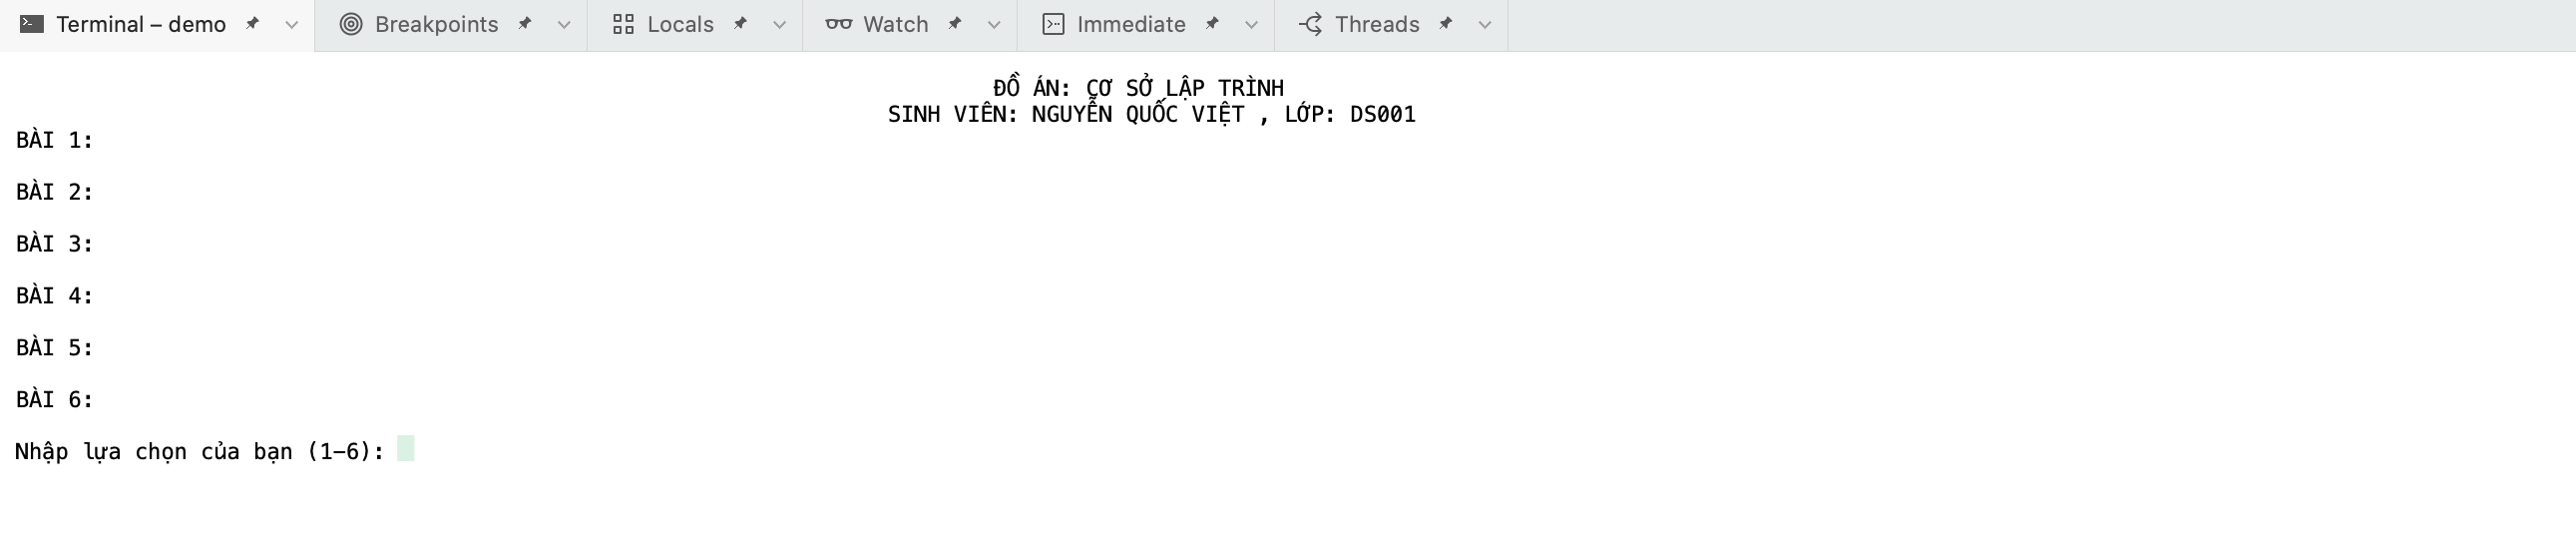
\includegraphics[width=17cm]{menu.png}
        \caption{Màn hình kết quả Menu}
    \end{figure}

Hiển thị kết quả bài 1, với lựa chọn người dúng là Búa, lựa chọn máy tính là Kéo
        \begin{figure}[!h]
        \centering
        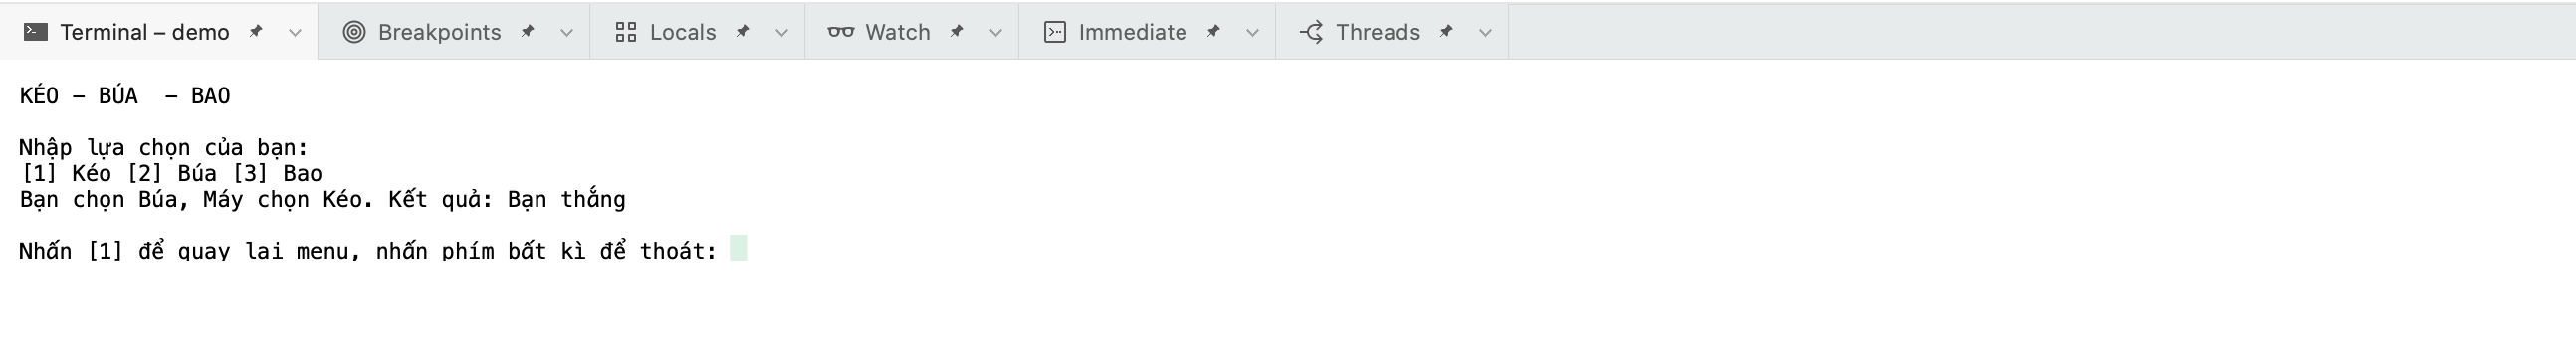
\includegraphics[width=17cm]{bai1.png}
        \caption{Màn hình kết quả bài 1}
    \end{figure}

Hiển thị kết quả bài 2, với số thứ tự là 42
        \begin{figure}[!h]
        \centering
        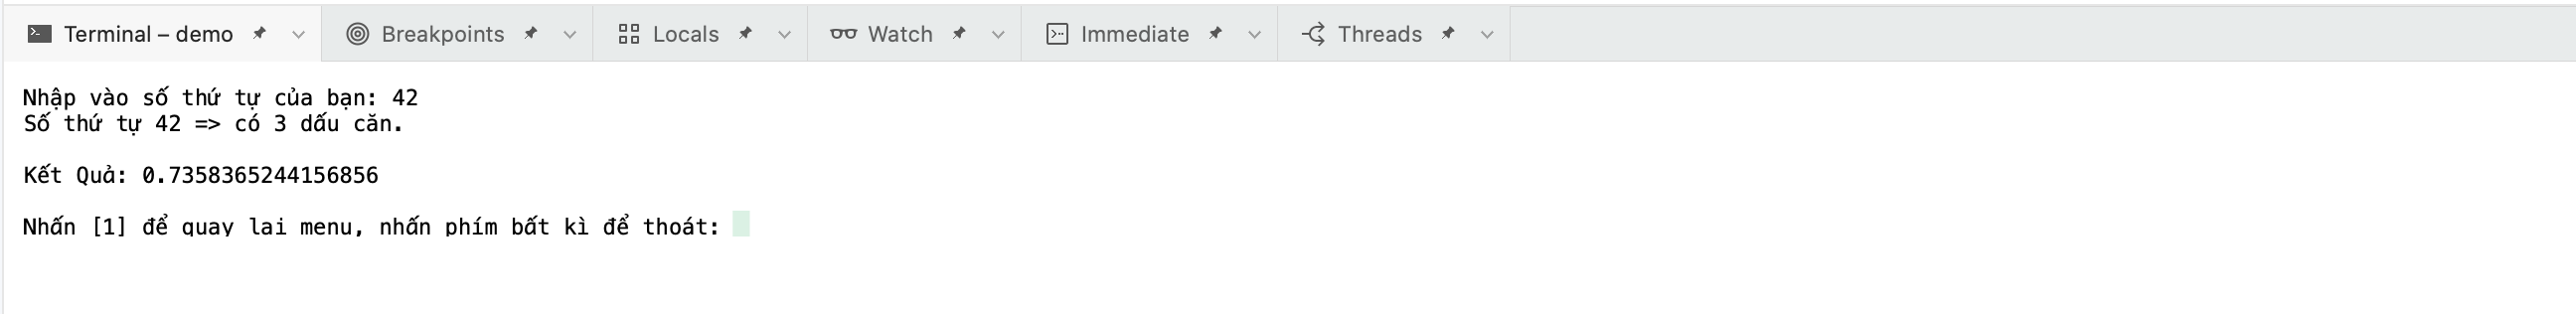
\includegraphics[width=17cm]{bai2.png}
        \caption{Màn hình kết quả bài 2}
    \end{figure}

Hiển thị kết quả bài 3, với đa thức bậc 4 và các hệ số lần lượt là: 1,2,3,4, hệ số tự do là 5 và $x=6$
        \begin{figure}[!h]
        \centering
        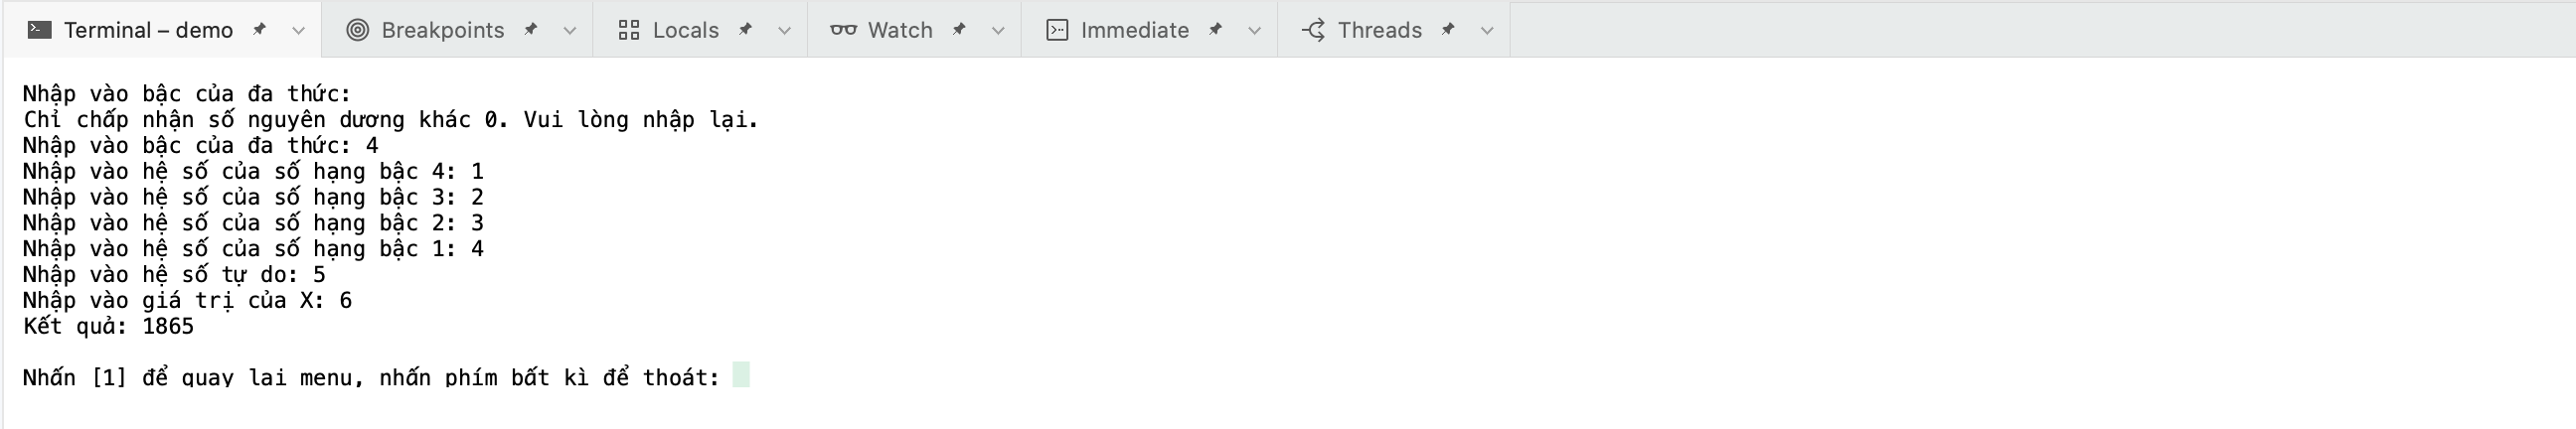
\includegraphics[width=17cm]{bai3.png}
        \caption{Màn hình kết quả bài 3}
    \end{figure}
    
\pagebreak
Hiển thị kết quả bài 4, với ma trận đầu vào là một ma trận $3 \times 3$ có dạng:
$ \begin{bmatrix}
1 & 0 & 1 \\
1 & 0 & 1 \\
1 & 0 & 1 
\end{bmatrix}  $

        \begin{figure}[!h]
        \centering
        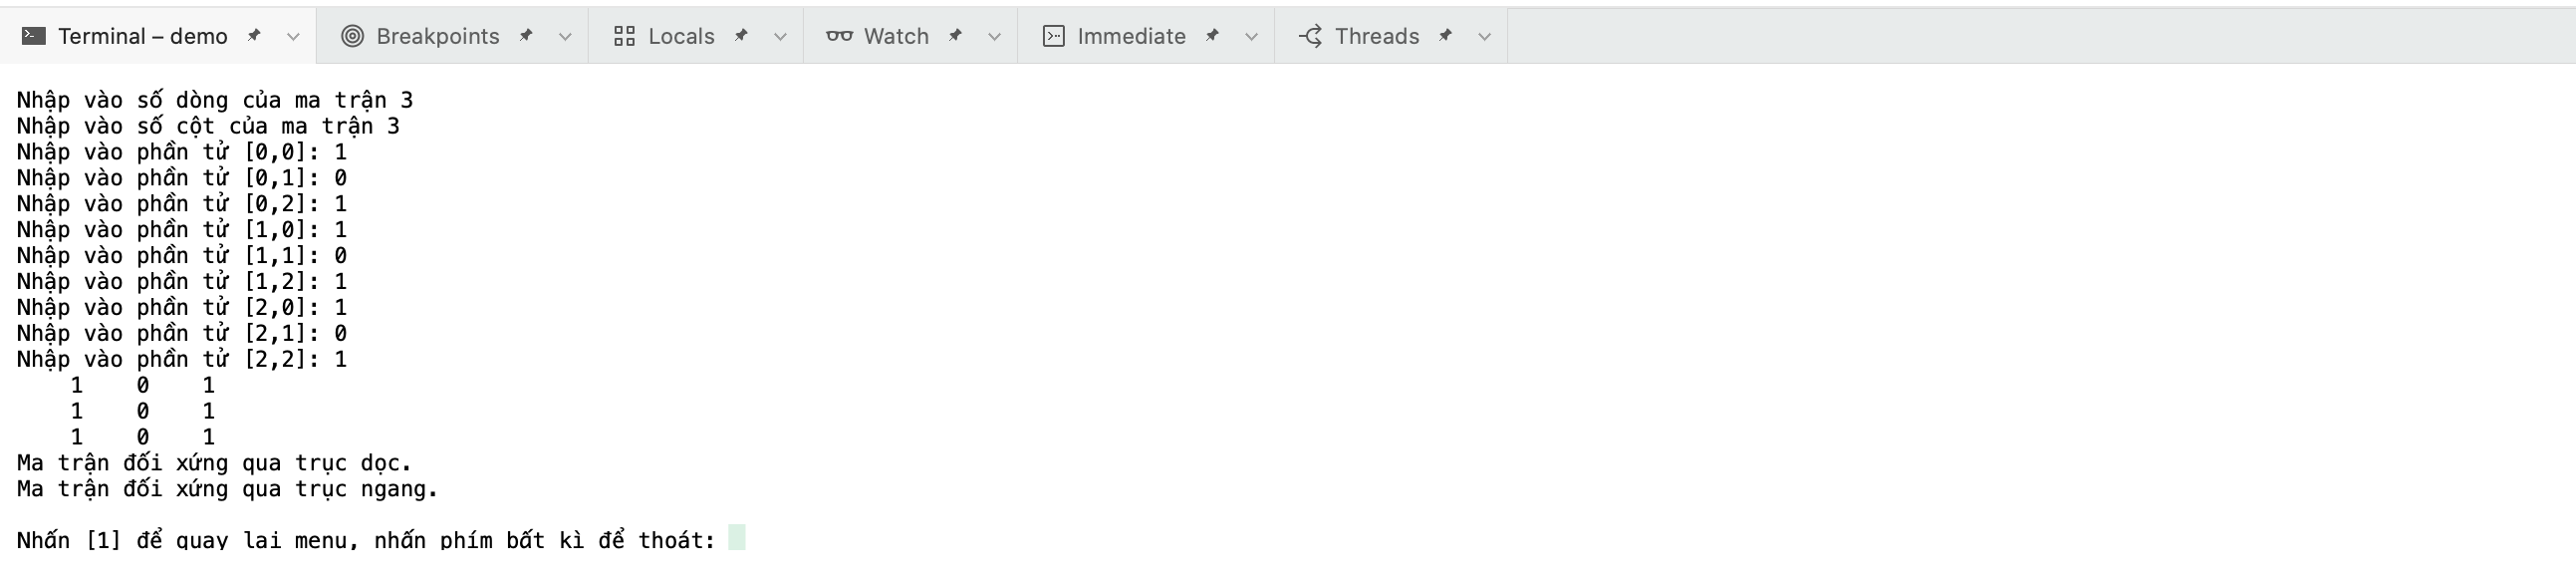
\includegraphics[width=17cm]{bai4.png}
        \caption{Màn hình kết quả bài 4}
    \end{figure}

Hiển thị kết quả bài 5, với xâu gốc $S$ = "Toi di hoc o truong dai hoc", xâu cần thay thế $S_1$ = "hoc", xâu thay thế $S_2$ = "di"
        \begin{figure}[!h]
        \centering
        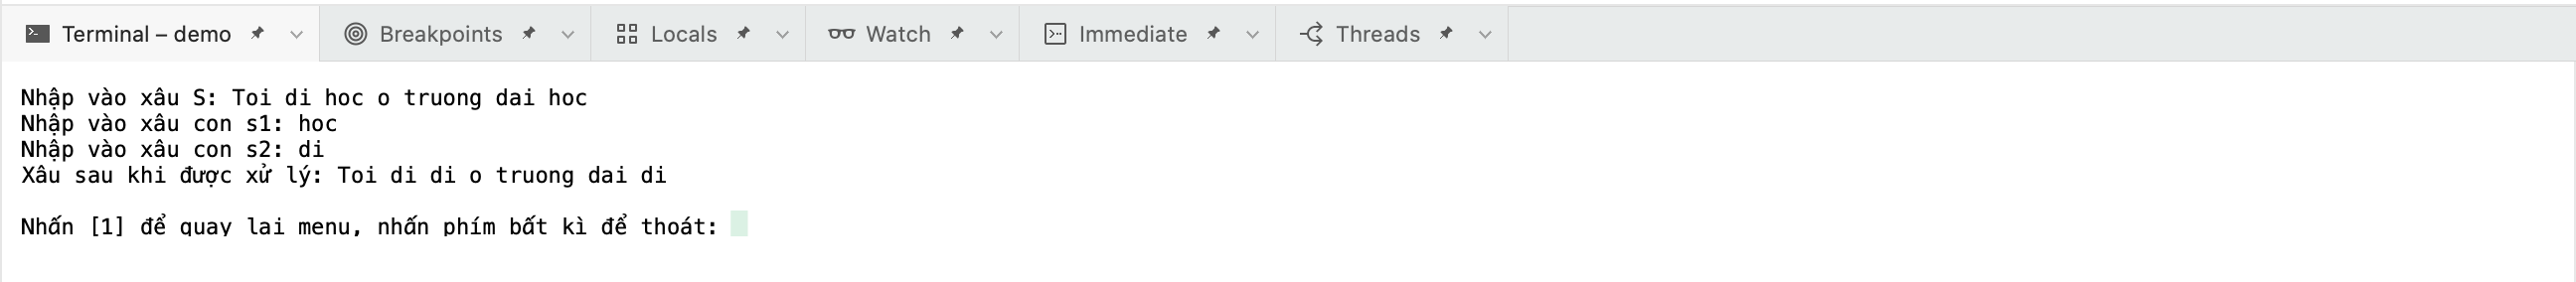
\includegraphics[width=17cm]{bai5.png}
        \caption{Màn hình kết quả bài 5}
    \end{figure}

Hiển thị kết quả bài 6, với thông tin hai sinh viên lần lượt là:
\begin{enumerate}
    \item Sinh viên 1
    \begin{itemize}
        \item Tên: Nguyễn Văn A
        \item Năm sinh: 2003
        \item Điểm trung bình: 8
    \end{itemize}
    \item Sinh viên 2
    \begin{itemize}
        \item Tên: Phạm Thị B
        \item Năm sinh: 2003
        \item Điểm trung bình: 9.5
    \end{itemize}
\end{enumerate}
        \begin{figure}[!h]
        \centering
        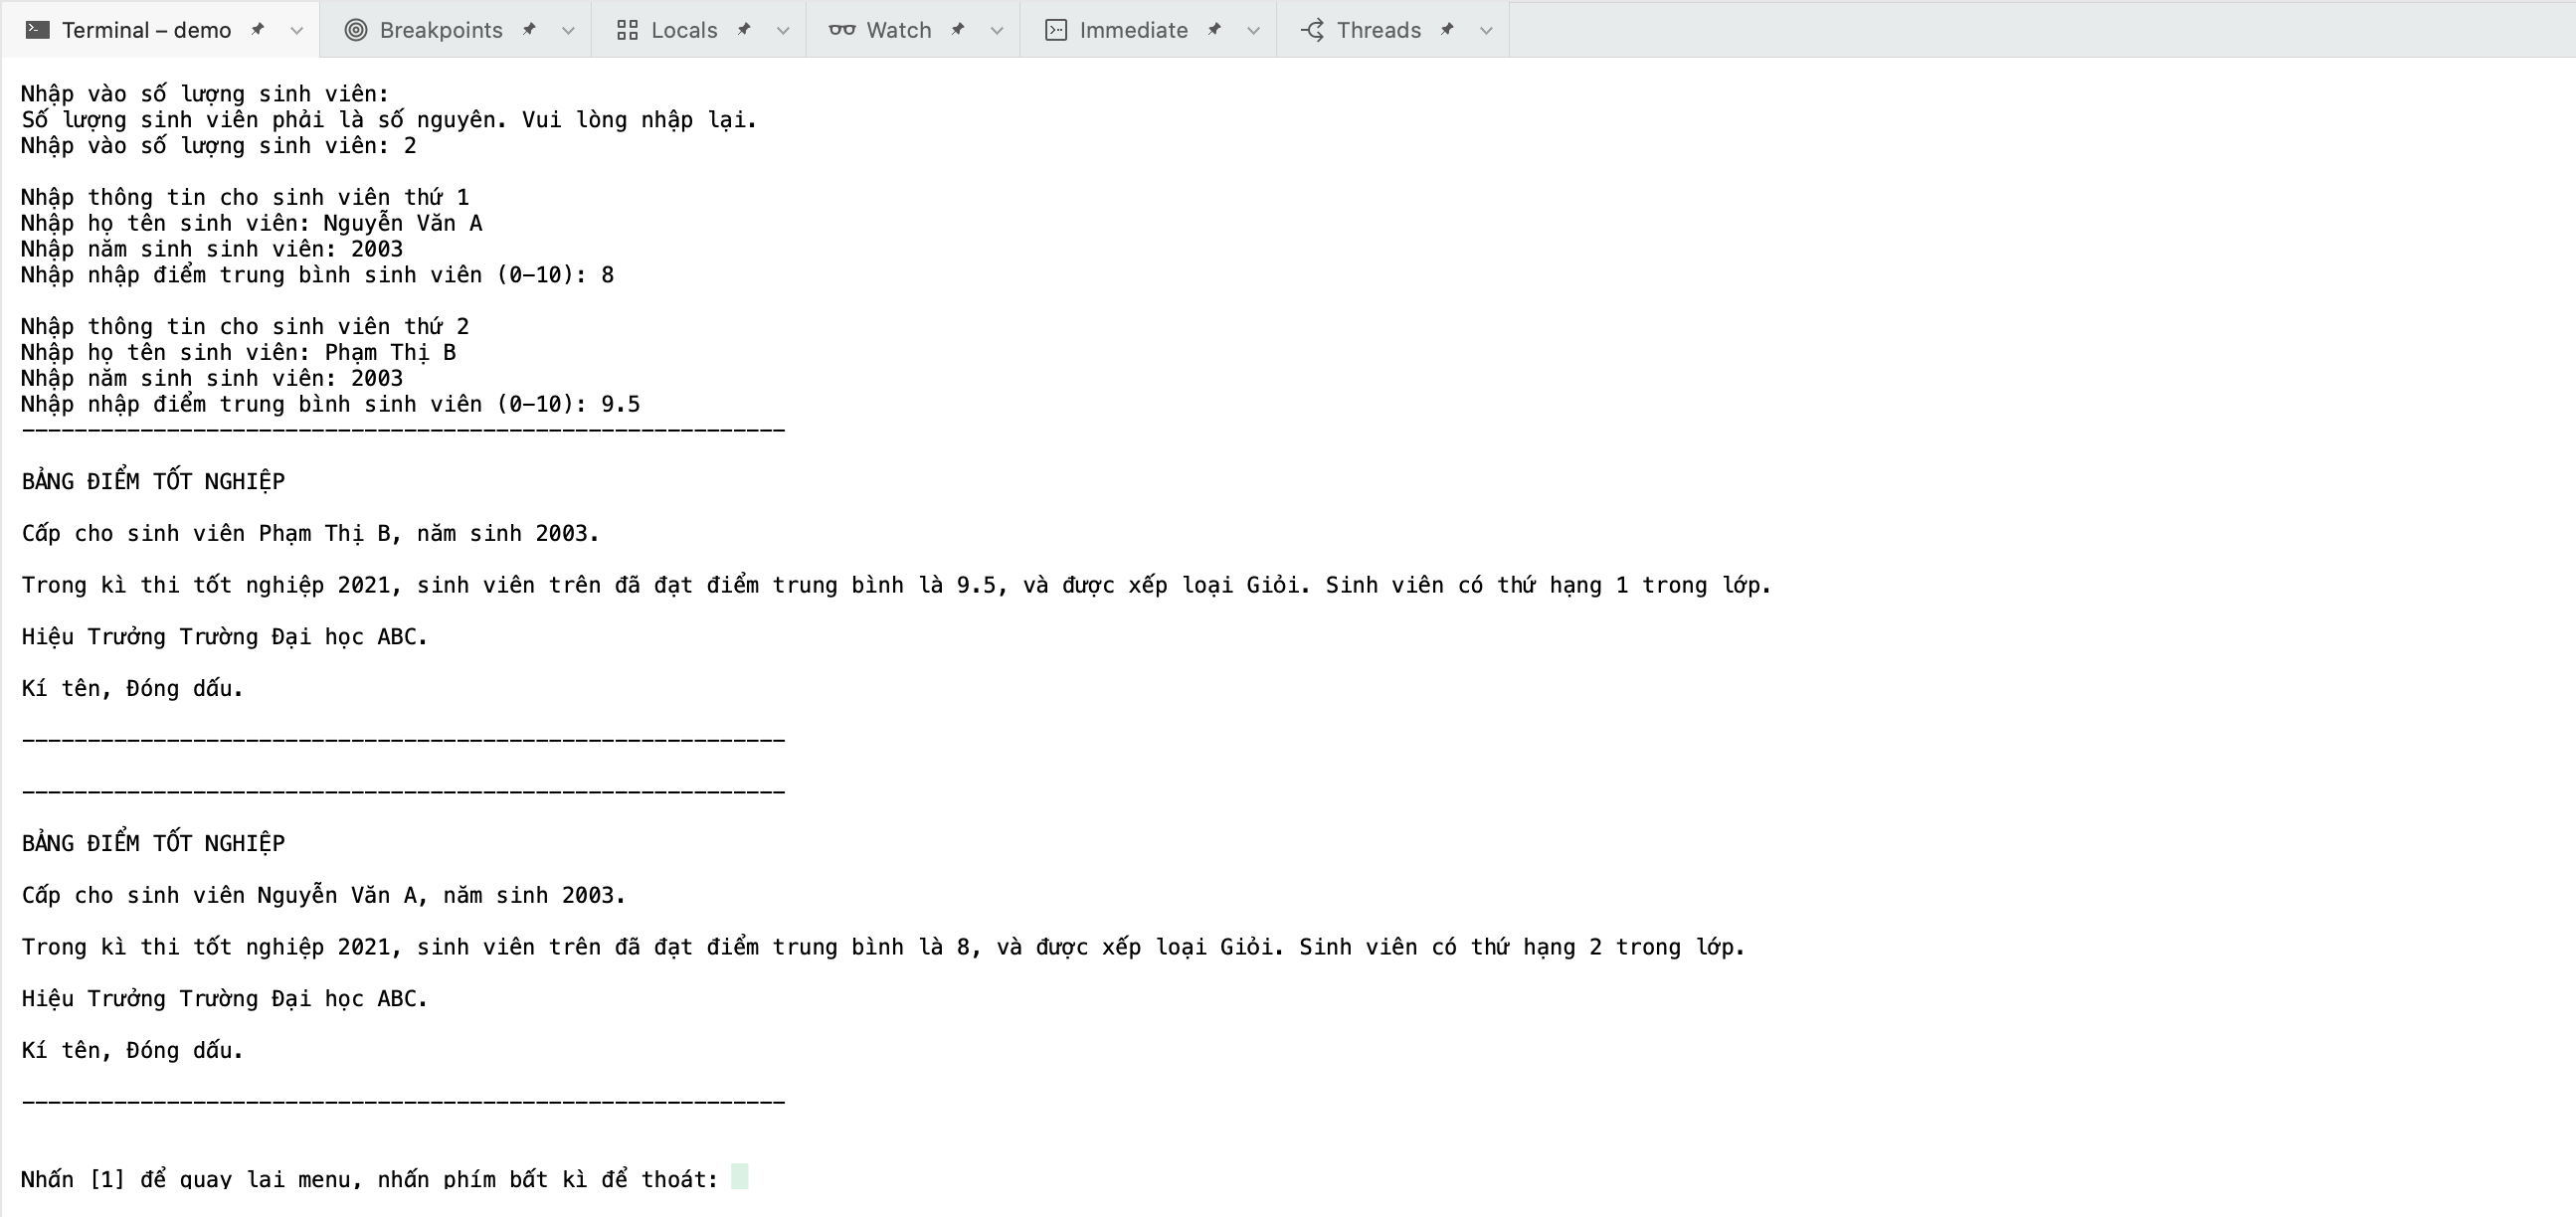
\includegraphics[width=17cm]{bai6.png}
        \caption{Màn hình kết quả bài 6}
    \end{figure}

\pagebreak
\section{PHỤ LỤC}
\textbf{Tạo menu người dùng chọn bài và in thông tin sinh viên}
\begin{itemize}
    \item Khai báo hàm \texttt{static void Main}
    \item In thông tin sinh viên:\\
    \texttt{Console.WriteLine("SINH VIÊN: NGUYỄN QUỐC VIỆT, LỚP: DS001);}\\
    \item Yêu cầu người dùng chọn bài. Xuất ra màn hình thông báo chọn bài.
    \item Dùng câu lệnh \texttt{switch-case} đễ dẫn đến hàm có bài tương ứng với thông tin người dùng đã nhập, nếu thông tin nhập vào không hợp lệ thì xuất thông báo "Lựa chọn của bạn không tồn tại. Vui lòng nhập lại."
    \item Xuất câu lệnh "Nhấn [1] để quay lại menu, nhấn phím bất kì để thoát: " và quay lại menu nếu người dùng nhấn 1, ngược lại thoát chương trình.
\end{itemize}

\textbf{Mã nguồn}
\begin{minted}[tabsize=2,breaklines,frame=lines,framesep=2mm,baselinestretch=1.2, bgcolor=LightGray, fontsize=\footnotesize, linenos]
{csharp}
        static void Main(string[] args)
        {
        start:
            Console.Clear();
            Console.OutputEncoding = System.Text.Encoding.Unicode;
            Console.InputEncoding = System.Text.Encoding.Unicode;
            string s = "44444444444444444444444444444444444444444444";
            Console.SetCursorPosition((Console.WindowWidth - s.Length) / 2, Console.CursorTop);
            Console.WriteLine("ĐỒ ÁN: CƠ SỞ LẬP TRÌNH");
            Console.SetCursorPosition((Console.WindowWidth - s.Length - 15) / 2, Console.CursorTop);
            Console.WriteLine("SINH VIÊN: NGUYỄN QUỐC VIỆT, LỚP: DS001");
            Console.WriteLine("BÀI 1:\n\nBÀI 2:\n\nBÀI 3:\n\nBÀI 4:\n\nBÀI 5:\n\nBÀI 6:\n");
        reinput_main:
            Console.Write("Nhập lựa chọn của bạn (1-6): ");
            ConsoleKeyInfo key;
            key = Console.ReadKey(true);
            int task;
            string num = key.KeyChar.ToString();
            if (int.TryParse(num, out task) == false)
            {
                Console.WriteLine("Lựa chọn của bạn không tồn tại. Vui lòng nhập lại.");
                goto reinput_main;
            }
            if (task > 0 & task < 7)
                switch (task)
                {
                    case 1: Console.WriteLine("Lựa chọn của bạn: Bài 1"); Thread.Sleep(1000); bai1(); break;
                    case 2: Console.WriteLine("Lựa chọn của bạn: Bài 2"); Thread.Sleep(1000); bai2(); break;
                    case 3: Console.WriteLine("Lựa chọn của bạn: Bài 3"); Thread.Sleep(1000); bai3(); break;
                    case 4: Console.WriteLine("Lựa chọn của bạn: Bài 4"); Thread.Sleep(1000); bai4(); break;
                    case 5: Console.WriteLine("Lựa chọn của bạn: Bài 5"); Thread.Sleep(1000); bai5(); break;
                    case 6: Console.WriteLine("Lựa chọn của bạn: Bài 6"); Thread.Sleep(1000); bai6(); break;

                }
            else
            {
                Console.WriteLine("Lựa chọn của bạn không tồn tại. Vui lòng nhập lại.");
                goto reinput_main;
            }

            Console.Write("\nNhấn [1] để quay lại menu, nhấn phím bất kì để thoát: ");
            key = Console.ReadKey(true);
            string input = key.KeyChar.ToString();
            if (input == "1")
                goto start;
            else
                goto end;
            end:;
        }
\end{minted}
 \pagebreak
\bibliography{cslt}
\bibliographystyle{apalike}
\cite{sharp_2015_microsoft,albahari_2022_c,arvindkumarbansal_2014_introduction,billwagner_c,srivastava2010shaping,price_2021_c,skeet_2019_c}
\end{document}


